\documentclass[11pt]{article}
\usepackage[a4paper,margin=2cm]{geometry}
\usepackage[T1]{fontenc}
\usepackage{lmodern,microtype}
\usepackage{amsmath,booktabs}
\usepackage[authoryear,round]{natbib}
\usepackage[hidelinks]{hyperref}
\usepackage{pgfplots}
\usepgfplotslibrary{groupplots,fillbetween}
\pgfplotsset{compat=1.18}
\usetikzlibrary{shapes.geometric}
\usepackage{caption}
\captionsetup{font=small,labelfont=bf}
\setlength{\textfloatsep}{12pt plus 2pt minus 4pt}
\setlength{\intextsep}{6pt plus 2pt minus 2pt}
\bibpunct{(}{)}{;}{a}{,}{,}

% Colours: TCGA-UT blue, BRACS orange.
\definecolor{cP}{HTML}{4575B4}
\definecolor{cS}{HTML}{91BFDB}
\definecolor{cI}{HTML}{FDAE61}
\definecolor{tcga}{HTML}{2166AC}
\definecolor{bracs}{HTML}{D6604D}

% Realized training class counts, sorted head to tail (exp-02 allocator; N = native shares of split 0, draw 0).
\pgfplotstableread{
rank r1 r2 r5 r10 r20 r50 r100 N
1 640 886 1278 1615 1973 2466 2843 1746
2 640 865 1209 1491 1780 2155 2426 1684
3 640 845 1144 1378 1605 1883 2070 1675
4 640 825 1082 1272 1448 1645 1766 1206
5 640 805 1024 1175 1305 1438 1506 1182
6 640 786 969 1086 1177 1256 1285 897
7 640 768 916 1003 1062 1098 1097 894
8 640 750 867 926 958 959 936 841
9 640 732 820 856 864 838 798 836
10 640 715 776 790 779 732 681 807
11 640 698 734 730 702 640 581 708
12 640 681 694 674 634 559 496 703
13 640 665 657 623 571 489 423 702
14 640 649 621 575 515 427 361 665
15 640 634 588 531 465 373 308 605
16 640 619 556 491 419 326 263 596
17 640 604 526 453 378 285 224 472
18 640 590 498 419 341 249 191 445
19 640 576 471 387 307 217 163 422
20 640 563 445 357 277 190 139 337
21 640 549 421 330 250 166 119 290
22 640 536 399 305 226 145 101 247
23 640 524 377 281 203 127 86 234
24 640 511 357 260 183 111 74 179
25 640 499 338 240 165 97 63 176
26 640 487 319 222 149 85 54 161
27 640 476 302 205 135 74 46 145
28 640 465 286 189 121 65 39 130
29 640 454 270 175 109 56 33 119
30 640 443 256 161 99 49 28 96
}\tcgacounts
\pgfplotstableread{
rank r1 r2 r5 r10 r20 r50 r100 N
1 320 441 622 766 908 1084 1206 678
2 320 392 476 522 551 565 560 556
3 320 350 364 356 335 294 260 459
4 320 312 278 242 203 153 120 176
5 320 278 213 165 123 80 56 129
6 320 247 163 112 75 42 26 127
7 320 220 124 77 45 22 12 115
}\bracscounts

\newcommand{\countlines}[1]{%
  \addplot[black,thick,mark=*,mark size=1pt] table[x=rank,y=r1]{#1};
  \addplot[red!80!black,thick,dashed,mark=square*,mark size=1pt] table[x=rank,y=N]{#1};
  \addplot[tcga,thick,mark=triangle*,mark size=1.4pt] table[x=rank,y=r100]{#1};}

\title{\vspace{-1cm}\LARGE Class Imbalance in Histopathology Patch Classification\vspace{-0.5em}}
\author{Yannik Queisler}
\date{September 25, 2026}

\begin{document}
\maketitle

\section{Motivation}
Histopathology datasets are long-tailed almost by construction. Common cancers and benign tissue dominate archives, while rare subtypes and atypical lesions, often diagnostically decisive, contribute few patients and patches. In convolutional neural networks, imbalance degrades classification, and the network absorbs the training class prior \citep{buda2018classImbalance}. In medical imaging, metrics dominated by the majority class can hide poor minority-class performance in both discrimination and calibration \citep{mosquera2024classImbalance}. Researchers continue to propose histopathology-specific models \citep{cong2022imbalancedHistopathology}. Pathology foundation models such as UNI and Virchow2 are commonly evaluated with linear classifiers trained on their frozen patch features \citep{chen2024uni,zimmermann2024virchow2}. Yet how much class imbalance costs such classifiers, and why, remains insufficiently measured in isolation.

Three questions guide this work. How much do discrimination and calibration degrade as the training class distribution becomes more skewed (Section~\ref{sec:effects})? What causes this damage, and why are some classes and tasks more vulnerable than others (Section~\ref{sec:cause})? How much of the damage can mitigation methods recover (Section~\ref{sec:mitigation})?

\section{Setup}
Multinomial logistic regression on Virchow2 patch features \citep{zimmermann2024virchow2} addresses two tasks: TCGA-UT, 30 cancer types \citep{komura2022universalEncoding}, and BRACS, 7 breast-lesion subtypes from normal tissue to invasive carcinoma \citep{brancati2022bracs}. Allocation conditions use the same patients per class (20 on TCGA-UT, 10 on BRACS) and total patch budget; only class shares change. An exponential profile sets the largest-to-smallest class ratio $\rho$ from 1 to 100 (Figure~\ref{fig:dist}). Class-to-rank assignment is randomized over 30 draws (3 splits $\times$ 10 draws); a native condition preserves each dataset's class shares. The outcome is \emph{damage}, $\Delta(\rho)=\mathrm{BA}(1)-\mathrm{BA}(\rho)$: the loss in test patient-macro balanced accuracy (BA) relative to the balanced condition, with paired bootstrap 95\% intervals. Damage counts as material from 1 percentage point (pp).

The encoder stays frozen when measuring damage and its causes. Mitigation methods that adapt the encoder fine-tune it through low-rank adaptation (LoRA) \citep{hu2022lora}. To rule out dependence on one encoder, the conditions at $\rho=10$ and $\rho=100$ are repeated on the same patients and patches with UNI2-h, the successor of UNI \citep{mahmoodlab2025uniRepo}.

\begin{figure}[!htb]
\centering
\begin{tikzpicture}
\begin{groupplot}[group style={group size=2 by 1,horizontal sep=1.3cm},
  width=0.5\textwidth,height=4.7cm,xlabel={Class rank (head $\to$ tail)},
  ymin=0,scaled y ticks=false,
  tick label style={font=\scriptsize},label style={font=\small},title style={font=\small},
  enlarge x limits=0.03]
\nextgroupplot[title={(a) TCGA-UT (30 classes, $T=19{,}200$)},ylabel={Training patches},xmin=1,xmax=30,
  legend style={font=\scriptsize,at={(0.98,0.97)},anchor=north east,draw=none,fill=none},
  legend cell align=left]
\countlines{\tcgacounts}
\legend{balanced ($\rho=1$),native ($\rho=18.1$),$\rho=100$}
\nextgroupplot[title={(b) BRACS (7 classes, $T=2{,}240$)},xmin=1,xmax=7,xtick={1,...,7},
  legend style={font=\scriptsize,at={(0.98,0.97)},anchor=north east,draw=none,fill=none},legend cell align=left]
\countlines{\bracscounts}
\legend{balanced ($\rho=1$),native ($\rho=6.7$),$\rho=100$}
\end{groupplot}
\end{tikzpicture}
\caption{Training class distributions sorted from head to tail: balanced, native shares of one split, and $\rho=100$. The tested ratios are $\rho\in\{1,2,5,10,20,50,100\}$; intermediate profiles lie between balanced and $\rho=100$. Class-to-rank assignment is randomized per draw. $T$: total training patch budget.}
\label{fig:dist}
\end{figure}

\section{Effects of class imbalance}
\label{sec:effects}
Balanced accuracy in the balanced condition reaches 72.1\% on TCGA-UT and 39.6\% on BRACS. Published evaluations show the same broad gap: region-of-interest (ROI)-level benchmarks report 59.5--67.5\% for UNI, Virchow2, and UNI2-h on the 32-class TCGA-UT task \citep{mahmoodlab2025uniRepo}, while slide-level linear probes score 31.8--48.1\% on BRACS \citep{vaidya2025threads}. TCGA-UT spans cancer types across organs, while BRACS separates breast lesions with similar morphology, such as atypical ductal hyperplasia (ADH) and ductal carcinoma in situ (DCIS) \citep{brancati2022bracs}. These evaluations make the gap plausible, though their training budgets and evaluation units differ. This study computes patient-macro balanced accuracy from patch predictions.

Imbalance damage differs strongly between the two tasks (Figure~\ref{fig:damage}a). On TCGA-UT, damage is small but accelerates as $\rho$ increases: 0.57 pp [0.30, 0.84] at $\rho=10$, reaching the 1-pp threshold at $\rho=20$ (1.01 pp [0.67, 1.36]) and 2.91 pp [2.48, 3.34] at $\rho=100$. On BRACS, damage appears at $\rho=2$ and grows steadily by about 1.15 pp per doubling of $\rho$: 1.15 pp [0.14, 2.35] at $\rho=2$, 4.02 pp [2.50, 5.66] at $\rho=10$, and 7.65 pp [5.77, 9.78] at $\rho=100$, a fifth of the balanced accuracy. The native allocations lie on their respective curves (1.18 pp [0.85, 1.48] on TCGA-UT and 4.05 pp [2.69, 5.57] on BRACS). Aggregate damage hides a large shift in recall from tail to head. At $\rho=100$, the TCGA-UT tail third loses 11.8 pp while the head gains 5.4 pp; on BRACS, the two tail classes drop from 38.7\% to 7.3\% recall.

Calibration deteriorates far more than accuracy (Figure~\ref{fig:damage}b). Expected calibration error (ECE), the average gap between the model's confidence and its accuracy, rises from 5.5 to 17.8 pp on TCGA-UT and from 12.3 to 35.7 pp on BRACS at $\rho=100$: the model becomes overconfident, but uniformly so. Temperature scaling divides all logits by one scalar fitted on validation data \citep{guo2017calibration}. This global confidence correction removes 92--96\% of the increase.

Replacing Virchow2 with UNI2-h changes the damage little. On TCGA-UT, UNI2-h's balanced baseline is 1.78 pp higher, and its damage at $\rho=100$ is 0.86 pp lower (97.5\% interval 0.40 to 1.33): a resolved difference, but below the 1-pp threshold. On BRACS, the difference is unresolved, and tail-class recall falls to about 9\% with both encoders.

\begin{figure}[t]
\centering
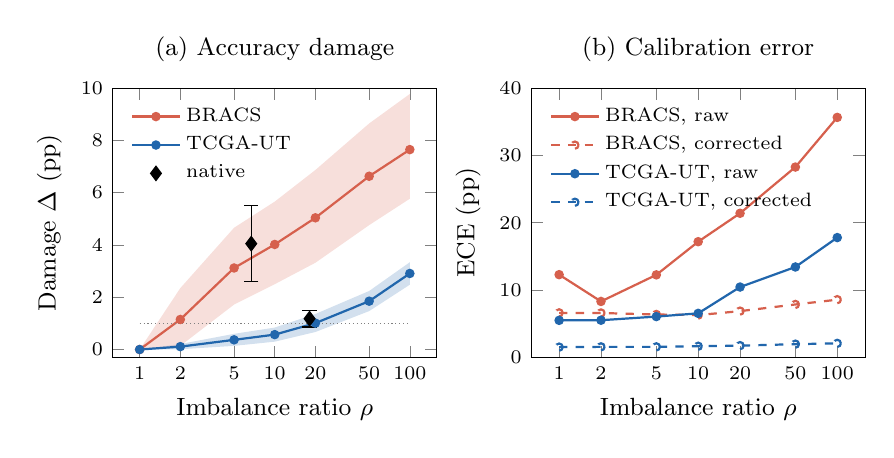
\begin{tikzpicture}
\begin{axis}[name=curve,title={(a) Accuracy damage},title style={font=\small},width=0.47\textwidth,height=5cm,xmode=log,log basis x=10,
  xtick={1,2,5,10,20,50,100},xticklabels={1,2,5,10,20,50,100},
  xlabel={Imbalance ratio $\rho$},ylabel={Damage $\Delta$ (pp)},ymin=-0.3,ymax=10,
  tick label style={font=\scriptsize},label style={font=\small},
  legend style={font=\scriptsize,at={(0.03,0.97)},anchor=north west,draw=none,fill=none},legend cell align=left]
\addplot[name path=tu,draw=none,forget plot] coordinates {(1,0)(2,0.21)(5,0.60)(10,0.84)(20,1.36)(50,2.24)(100,3.34)};
\addplot[name path=tl,draw=none,forget plot] coordinates {(1,0)(2,0.01)(5,0.14)(10,0.30)(20,0.67)(50,1.47)(100,2.48)};
\addplot[tcga,fill opacity=0.2,forget plot] fill between[of=tu and tl];
\addplot[name path=bu,draw=none,forget plot] coordinates {(1,0)(2,2.35)(5,4.66)(10,5.66)(20,6.87)(50,8.65)(100,9.78)};
\addplot[name path=bl,draw=none,forget plot] coordinates {(1,0)(2,0.14)(5,1.72)(10,2.50)(20,3.32)(50,4.76)(100,5.77)};
\addplot[bracs,fill opacity=0.2,forget plot] fill between[of=bu and bl];
\addplot[bracs,thick,mark=*,mark size=1.3pt] coordinates {(1,0)(2,1.15)(5,3.12)(10,4.02)(20,5.04)(50,6.63)(100,7.65)};
\addlegendentry{BRACS}
\addplot[tcga,thick,mark=*,mark size=1.3pt] coordinates {(1,0)(2,0.11)(5,0.37)(10,0.57)(20,1.01)(50,1.85)(100,2.91)};
\addlegendentry{TCGA-UT}
\addplot[only marks,mark=diamond*,mark size=2.6pt,black,error bars/.cd,y dir=both,y explicit]
  coordinates {(18.1,1.18) +- (0,0.32) (6.7,4.05) +- (0,1.45)};
\addlegendentry{native}
\draw[densely dotted,gray] (axis cs:1,1) -- (axis cs:100,1);
\end{axis}
\begin{axis}[at={(curve.east)},title={(b) Calibration error},title style={font=\small},anchor=west,xshift=1.2cm,width=0.48\textwidth,height=5cm,
  xmode=log,log basis x=10,xtick={1,2,5,10,20,50,100},xticklabels={1,2,5,10,20,50,100},
  xlabel={Imbalance ratio $\rho$},ylabel={ECE (pp)},ymin=0,ymax=40,
  tick label style={font=\scriptsize},label style={font=\small},
  legend style={font=\scriptsize,at={(0.03,0.97)},anchor=north west,draw=none,fill=none},legend cell align=left]
\addplot[bracs,thick,mark=*,mark size=1.3pt] coordinates {(1,12.29)(2,8.31)(5,12.26)(10,17.19)(20,21.41)(50,28.28)(100,35.66)};
\addlegendentry{BRACS, raw}
\addplot[bracs,thick,dashed,mark=o,mark size=1.3pt] coordinates {(1,6.61)(2,6.59)(5,6.37)(10,6.28)(20,6.87)(50,7.86)(100,8.57)};
\addlegendentry{BRACS, corrected}
\addplot[tcga,thick,mark=*,mark size=1.3pt] coordinates {(1,5.50)(2,5.52)(5,6.06)(10,6.54)(20,10.45)(50,13.43)(100,17.80)};
\addlegendentry{TCGA-UT, raw}
\addplot[tcga,thick,dashed,mark=o,mark size=1.3pt] coordinates {(1,1.52)(2,1.56)(5,1.56)(10,1.65)(20,1.74)(50,1.96)(100,2.08)};
\addlegendentry{TCGA-UT, corrected}
\end{axis}
\end{tikzpicture}
\caption{(a) Balanced-accuracy damage versus $\rho$ with 95\% bands; diamonds mark native class shares, dotted line the 1-pp threshold. (b) Expected calibration error (ECE) of the raw predicted probabilities (solid) and after a single global confidence correction fitted on validation data (dashed).}
\label{fig:damage}
\end{figure}

\section{Causes of class imbalance damage}
\label{sec:cause}
Two questions explain the damage. The first is which changes in the training data cause it (Section~\ref{sec:sources}). The second is why the same imbalance ratio costs more for some rare classes than for others (Section~\ref{sec:vulnerable}).

\subsection{Sources of damage}
\label{sec:sources}
When a tail class receives fewer training patches, two things change. Its errors contribute less often to the training loss, so common classes have more influence on the fitted decision boundary. This is the \emph{frequency} effect: how strongly each class's available examples shape the classifier. The model also sees fewer distinct tail patches, only one or two per patient at $\rho=100$, so it has less evidence about how that class varies. This is the \emph{support} effect: giving those few patches more weight cannot supply the missing examples.

The conditions in Table~\ref{tab:conditions} separate these effects. F keeps all patches from the balanced condition but gives head classes more weight, isolating the frequency effect. S keeps the sparse patches from the imbalanced condition but weights classes equally, isolating the support effect. The ratio condition r combines both effects. The interaction $I=\Delta_\mathrm{r}-\Delta_\mathrm{F}-\Delta_\mathrm{S}$ measures any additional damage when both occur together.

\begin{figure}[!htb]
\begin{minipage}[c]{0.48\textwidth}
\centering\small
\setlength{\tabcolsep}{3pt}
\begin{tabular}{@{}lcc@{}}
\toprule
Class influence & Many tail patches & Few tail patches \\
\midrule
Equal & balanced (ref.) & S: support only \\
Head-favoured & F: frequency only & r: ratio (both) \\
\bottomrule
\end{tabular}
\captionof{table}{Four training conditions separate the effect of unequal class influence (frequency) from the effect of fewer tail examples (support) at each $\rho$.}
\label{tab:conditions}
\end{minipage}\hfill
\begin{minipage}[c]{0.48\textwidth}
\centering
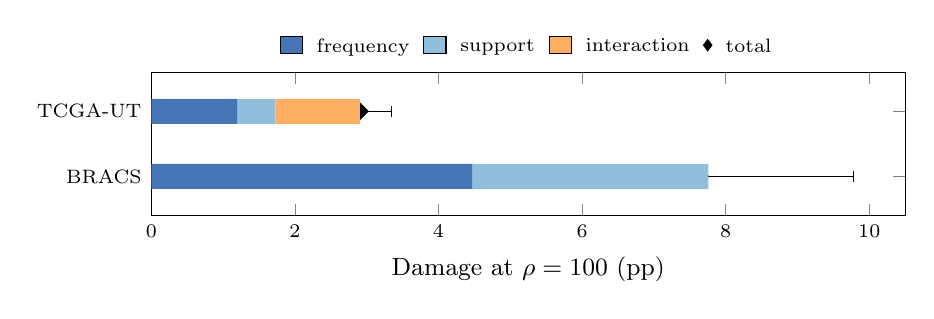
\begin{tikzpicture}
\begin{axis}[xbar stacked,width=0.92\linewidth,height=3.4cm,bar width=9pt,
  xmin=0,xmax=10.5,xlabel={Damage at $\rho=100$ (pp)},
  ytick={1,2},yticklabels={BRACS,TCGA-UT},ymin=0.4,ymax=2.6,
  tick label style={font=\scriptsize},label style={font=\small},
  legend style={font=\scriptsize,at={(0.5,1.03)},anchor=south,draw=none,fill=none,legend columns=4,column sep=3pt},
  legend cell align=left]
\addplot[fill=cP,draw=none] coordinates {(4.47,1) (1.20,2)};
\addlegendentry{frequency}
\addplot[fill=cS,draw=none] coordinates {(3.29,1) (0.53,2)};
\addlegendentry{support}
\addplot[fill=cI,draw=none] coordinates {(0,1) (1.18,2)};
\addlegendentry{interaction}
\addlegendimage{only marks,mark=diamond*,black}
\addlegendentry{total}
% Totals drawn outside the stack (an addplot here would stack onto the bars).
\draw[black,thin] (axis cs:5.77,1) -- (axis cs:9.78,1);
\draw[black,thin] ([yshift=-2pt]axis cs:5.77,1) -- ([yshift=2pt]axis cs:5.77,1);
\draw[black,thin] ([yshift=-2pt]axis cs:9.78,1) -- ([yshift=2pt]axis cs:9.78,1);
\node[diamond,fill=black,inner sep=1.6pt] at (axis cs:7.65,1) {};
\draw[black,thin] (axis cs:2.48,2) -- (axis cs:3.34,2);
\draw[black,thin] ([yshift=-2pt]axis cs:2.48,2) -- ([yshift=2pt]axis cs:2.48,2);
\draw[black,thin] ([yshift=-2pt]axis cs:3.34,2) -- ([yshift=2pt]axis cs:3.34,2);
\node[diamond,fill=black,inner sep=1.6pt] at (axis cs:2.91,2) {};
\end{axis}
\end{tikzpicture}
\caption{Damage at $\rho=100$ by component; diamonds give the total with its 95\% interval.}
\label{fig:decomp}
\end{minipage}
\end{figure}

\noindent The damage components differ between tasks (Figure~\ref{fig:decomp}). On TCGA-UT, the frequency effect accounts for damage at moderate ratios (0.73 of 1.01 pp at $\rho=20$), while sparse tail support alone costs nothing. At $\rho=100$, the two effects compound: frequency 1.20 pp [0.87, 1.53], support 0.53 pp [0.36, 0.70], and a positive interaction of 1.18 pp [1.00, 1.37]. On BRACS, both factors are material at $\rho=100$: frequency 4.47 pp [2.84, 6.30] and support 3.29 pp [1.99, 4.67]. Their sum matches the total damage. The interaction is near zero, $-0.11$ pp, but its interval [$-1.74$, 1.36] cannot rule out compounding of up to 1.4 pp. Sparse tail support alone costs BRACS more than total TCGA-UT imbalance damage.

\subsection{Vulnerable classes}
\label{sec:vulnerable}
On BRACS, rotating every class through every rank shows that easy classes cost most when rare. Damage at $\rho=100$ ranges from 5.73 pp (usual ductal hyperplasia, UDH, in the tail) to 9.99 pp (invasive carcinoma), because a class with high balanced recall has the most to lose (Figure~\ref{fig:order}a).

On TCGA-UT, a class is especially vulnerable when it receives few patches but a frequent confusion partner receives many. A score built from the balanced model's confusion rates ordered new class-to-rank assignments by damage. The score was chosen after exploratory checks on the same stored outputs and uses test predictions, so this shows the mechanism on these patients and is not an out-of-sample prediction. The assignment ranked most damaging costs 4.51 pp (a lower bound on the worst case, found by hill climbing), the least damaging 1.34 pp, and random assignments 2.91 pp (Figure~\ref{fig:order}b). Reversing the most damaging assignment preserves pairwise rank gaps but lowers damage by 1.11 pp [0.47, 1.73]. Damage is therefore greatest when the class prone to confusion is the rarer one.

\begin{figure}[!htb]
\centering
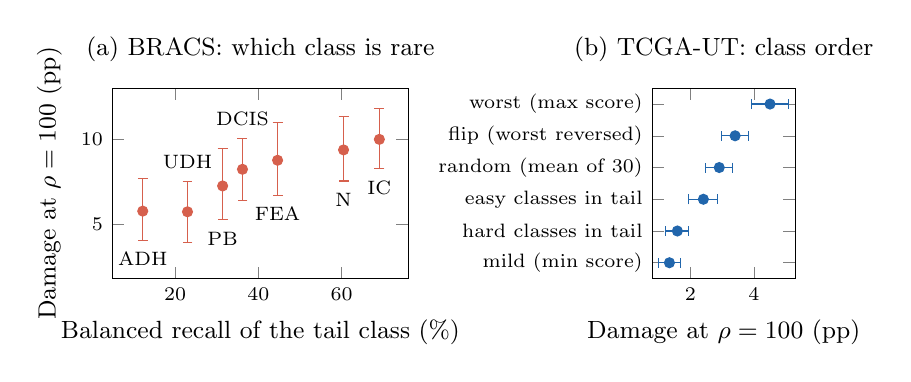
\begin{tikzpicture}
\begin{axis}[name=bracsorder,title={(a) BRACS: which class is rare},title style={font=\small},
  width=0.44\textwidth,height=4cm,xmin=5,xmax=76,ymin=1.8,ymax=13,clip=false,
  xlabel={Balanced recall of the tail class (\%)},ylabel={Damage at $\rho=100$ (pp)},
  tick label style={font=\scriptsize},label style={font=\small}]
\addplot[only marks,mark=*,bracs,mark size=1.8pt,error bars/.cd,y dir=both,y explicit]
  coordinates {(12.23,5.77) -= (0,1.71) += (0,1.92) (22.98,5.73) -= (0,1.80) += (0,1.79) (31.42,7.25) -= (0,1.99) += (0,2.19) (36.19,8.23) -= (0,1.81) += (0,1.82) (44.62,8.76) -= (0,2.05) += (0,2.24) (60.47,9.37) -= (0,1.83) += (0,1.95) (69.07,9.99) -= (0,1.73) += (0,1.81)};
\node[font=\scriptsize,below=1pt] at (axis cs:12.23,4.06) {ADH};
\node[font=\scriptsize,above=1pt] at (axis cs:22.98,7.52) {UDH};
\node[font=\scriptsize,below=1pt] at (axis cs:31.42,5.26) {PB};
\node[font=\scriptsize,above=1pt] at (axis cs:36.19,10.05) {DCIS};
\node[font=\scriptsize,below=1pt] at (axis cs:44.62,6.71) {FEA};
\node[font=\scriptsize,below=1pt] at (axis cs:60.47,7.54) {N};
\node[font=\scriptsize,below=1pt] at (axis cs:69.07,8.26) {IC};
\end{axis}
\begin{axis}[at={(bracsorder.east)},anchor=west,xshift=3.1cm,title={(b) TCGA-UT: class order},title style={font=\small},
  width=0.28\textwidth,height=4cm,xmin=0.8,xmax=5.3,ymin=0.5,ymax=6.5,
  ytick={1,...,6},yticklabels={mild (min score),hard classes in tail,easy classes in tail,random (mean of 30),flip (worst reversed),worst (max score)},
  xlabel={Damage at $\rho=100$ (pp)},tick label style={font=\scriptsize},label style={font=\small}]
\addplot[only marks,mark=*,tcga,mark size=1.8pt,error bars/.cd,x dir=both,x explicit]
  coordinates {(1.34,1) -= (0.34,0) += (0.35,0)
               (1.59,2) -= (0.37,0) += (0.36,0)
               (2.41,3) -= (0.46,0) += (0.44,0)
               (2.91,4) -= (0.43,0) += (0.43,0)
               (3.41,5) -= (0.43,0) += (0.43,0)
               (4.51,6) -= (0.58,0) += (0.57,0)};
\end{axis}
\end{tikzpicture}
\caption{Damage at $\rho=100$ with 95\% intervals. (a) BRACS tail-class identity versus balanced recall (Spearman correlation 0.96, $n=7$). ADH: atypical ductal hyperplasia; UDH: usual ductal hyperplasia; PB: pathological benign; DCIS: ductal carcinoma in situ; FEA: flat epithelial atypia; N: normal; IC: invasive carcinoma. (b) TCGA-UT class-to-rank assignments.}
\label{fig:order}
\end{figure}

\section{Mitigation of class imbalance damage}
\label{sec:mitigation}
Section~\ref{sec:cause} traced the damage to the frequency and support effects. This section asks how much of it established long-tailed methods recover compared with standard cross-entropy (CE) training. Six methods cover the three families of \citet{krawczyk2016learning} (Table~\ref{tab:methods}). Data-level methods change the training data, algorithm-level methods change the loss or the decision rule, and hybrid methods do both.

Several of these methods act on the learned representation, not only on the classifier. The encoder is therefore adapted through LoRA together with a linear head. The patients, patch budgets, and class-to-rank assignments match those in Section~\ref{sec:effects}. CE and each method are trained at $\rho=100$, $\rho=50$, and native shares, and a CE model trained on the balanced allocation provides the undamaged reference. Each method except cRT has one control parameter that sets how strongly it acts, such as the scale of the logit adjustment or the probability that CUDA augments a patch; it is selected per draw on validation patients.

Under LoRA, CE loses 4.95 pp [3.25, 6.74] on BRACS and 1.56 pp [1.17, 1.94] on TCGA-UT at $\rho=100$. Recovery is measured against this LoRA-specific damage, not the frozen-readout damage of Section~\ref{sec:effects}; the BRACS figure is lower mainly because the adapted balanced reference is weaker (Section~\ref{sec:limits}). A method's \emph{recovery} is its gain in balanced accuracy over CE at the same allocation; its \emph{share} is recovery divided by CE's damage. Methods whose effect on balanced data is not zero by construction are also fitted on the balanced allocation. Recovery minus this \emph{balanced gain} is the part that corrects the imbalance. Results refer to Virchow2 and $\rho=100$ unless stated otherwise.

\begin{table}[!htb]
\centering\small
\begin{tabular}{@{}llp{0.5\textwidth}@{}}
\toprule
Family & Method & What changes \\
\midrule
Data & Balanced sampling \citep{kang2020decouplingRepresentation} & Every class is drawn equally often. \\
 & CUDA \citep{ahn2023cuda} & Image patches are augmented per class, more strongly once the model has learned the class. \\
\addlinespace
Algorithm & Logit adjustment \citep{menon2021longTail} & The training class prior is subtracted from the class scores, in the loss or after training. \\
 & DisAlign \citep{zhang2021distributionAlignment} & A loss that weights rare classes more trains a per-class score correction. \\
\addlinespace
Hybrid & cRT \citep{kang2020decouplingRepresentation} & The head is refitted with balanced sampling. \\
 & GCL \citep{li2022gaussianClouded} & Random noise lowers the scores of rarer classes more during training; optionally, the head is then refitted with near-balanced sampling. \\
\bottomrule
\end{tabular}
\caption{The six mitigation methods change the data, the learner, or both. Logit adjustment is tested in the loss and after training, GCL with and without the head refit, giving eight variants. CUDA: curriculum of data augmentation; DisAlign: distribution alignment; cRT: classifier re-training; GCL: Gaussian clouded logit adjustment.}
\label{tab:methods}
\end{table}

\begin{figure}[!htb]
\centering
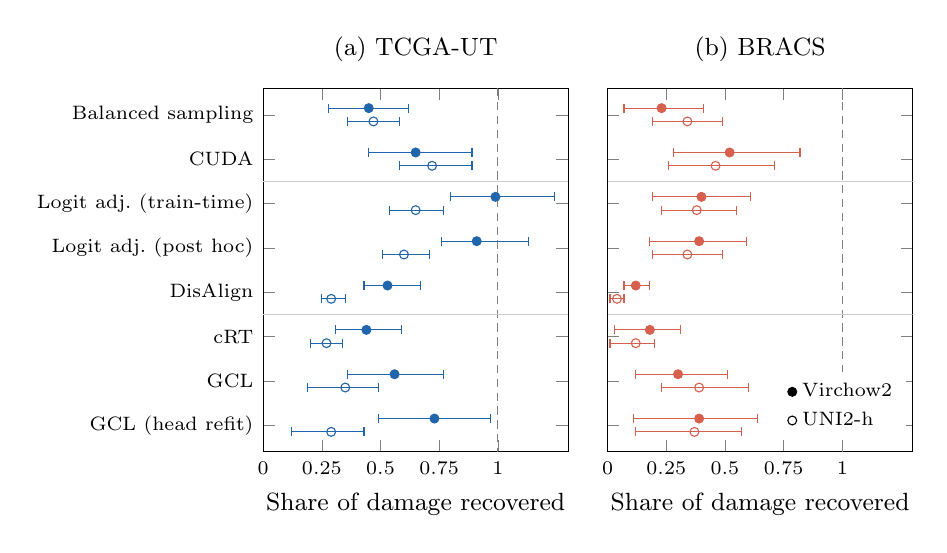
\begin{tikzpicture}
\begin{groupplot}[group style={group size=2 by 1,horizontal sep=0.5cm,yticklabels at=edge left},
  width=0.45\textwidth,height=6.2cm,xmin=0,xmax=1.3,xtick={0,0.25,0.5,0.75,1},
  xlabel={Share of damage recovered},ymin=0.4,ymax=8.6,y dir=reverse,ytick={1,...,8},
  yticklabels={Balanced sampling,CUDA,Logit adj.\ (train-time),Logit adj.\ (post hoc),DisAlign,cRT,GCL,GCL (head refit)},
  tick label style={font=\scriptsize},label style={font=\small},title style={font=\small},
  legend style={font=\scriptsize,at={(0.98,0.03)},anchor=south east,draw=none,fill=white},legend cell align=left]
\nextgroupplot[title={(a) TCGA-UT}]
\draw[densely dashed,gray] (axis cs:1,0.4) -- (axis cs:1,8.6);
\draw[gray!40] (axis cs:0,2.5) -- (axis cs:1.3,2.5) (axis cs:0,5.5) -- (axis cs:1.3,5.5);
\addplot[only marks,mark=*,tcga,mark size=1.6pt,error bars/.cd,x dir=both,x explicit,error bar style={tcga}]
  coordinates {(0.45,0.85) -= (0.17,0) += (0.17,0) (0.65,1.85) -= (0.20,0) += (0.24,0) (0.99,2.85) -= (0.19,0) += (0.25,0) (0.91,3.85) -= (0.15,0) += (0.22,0) (0.53,4.85) -= (0.10,0) += (0.14,0) (0.44,5.85) -= (0.13,0) += (0.15,0) (0.56,6.85) -= (0.20,0) += (0.21,0) (0.73,7.85) -= (0.24,0) += (0.24,0)};
\addplot[only marks,mark=o,tcga,mark size=1.6pt,error bars/.cd,x dir=both,x explicit,error bar style={tcga}]
  coordinates {(0.47,1.15) -= (0.11,0) += (0.11,0) (0.72,2.15) -= (0.14,0) += (0.17,0) (0.65,3.15) -= (0.11,0) += (0.12,0) (0.60,4.15) -= (0.09,0) += (0.11,0) (0.29,5.15) -= (0.04,0) += (0.06,0) (0.27,6.15) -= (0.07,0) += (0.07,0) (0.35,7.15) -= (0.16,0) += (0.14,0) (0.29,8.15) -= (0.17,0) += (0.14,0)};
\nextgroupplot[title={(b) BRACS}]
\draw[densely dashed,gray] (axis cs:1,0.4) -- (axis cs:1,8.6);
\draw[gray!40] (axis cs:0,2.5) -- (axis cs:1.3,2.5) (axis cs:0,5.5) -- (axis cs:1.3,5.5);
\addplot[forget plot,only marks,mark=*,bracs,mark size=1.6pt,error bars/.cd,x dir=both,x explicit,error bar style={bracs}]
  coordinates {(0.23,0.85) -= (0.16,0) += (0.18,0) (0.52,1.85) -= (0.24,0) += (0.30,0) (0.40,2.85) -= (0.21,0) += (0.21,0) (0.39,3.85) -= (0.21,0) += (0.20,0) (0.12,4.85) -= (0.05,0) += (0.06,0) (0.18,5.85) -= (0.15,0) += (0.13,0) (0.30,6.85) -= (0.18,0) += (0.21,0) (0.39,7.85) -= (0.28,0) += (0.25,0)};
\addplot[forget plot,only marks,mark=o,bracs,mark size=1.6pt,error bars/.cd,x dir=both,x explicit,error bar style={bracs}]
  coordinates {(0.34,1.15) -= (0.15,0) += (0.15,0) (0.46,2.15) -= (0.20,0) += (0.25,0) (0.38,3.15) -= (0.15,0) += (0.17,0) (0.34,4.15) -= (0.15,0) += (0.15,0) (0.04,5.15) -= (0.03,0) += (0.03,0) (0.12,6.15) -= (0.11,0) += (0.08,0) (0.39,7.15) -= (0.16,0) += (0.21,0) (0.37,8.15) -= (0.25,0) += (0.20,0)};
\addlegendimage{only marks,mark=*,black,mark size=1.6pt}
\addlegendentry{Virchow2}
\addlegendimage{only marks,mark=o,black,mark size=1.6pt}
\addlegendentry{UNI2-h}
\end{groupplot}
\end{tikzpicture}
\caption{Only logit adjustment on TCGA-UT with Virchow2 recovers the full damage; on BRACS no method recovers much more than half of it. Each method's share of CE damage recovered at $\rho=100$, with paired 95\% intervals, for Virchow2 (filled) and UNI2-h (hollow) on the same patients and patches. The dashed line marks full recovery. Grey lines separate the data-level, algorithm-level, and hybrid families of Table~\ref{tab:methods}.}
\label{fig:recovery}
\end{figure}

\subsection{What mitigation achieves}
\label{sec:helps}
\textbf{1. Cheap fixes already recover much of the damage.}
Logit adjustment removes the training prior from the class scores \citep{menon2021longTail}. Applied to the CE model after training, it needs no retraining and recovers as much as its train-time form: 1.41 against 1.54 pp on TCGA-UT and 1.94 against 1.96 pp on BRACS. On TCGA-UT this is essentially the full damage (Figure~\ref{fig:recovery}a). The train-time share is 0.99 [0.80, 1.24], and recall of the tail third of classes rises from 61.2\% to 69.4\%, against 71.6\% when balanced. On BRACS, both forms recover about two-fifths (Figure~\ref{fig:recovery}b). Balanced sampling, which changes only how often each class is drawn, recovers at least 1 pp in three of the four dataset--encoder settings.

\smallskip\noindent\textbf{2. Augmentation improves the model in general.}
CUDA recovers 0.46 to 0.72 of the damage across the four settings, the largest share in all but TCGA-UT with Virchow2, where logit adjustment recovers more. Most of this gain does not depend on imbalance: CUDA also improves the balanced model, by 0.81 pp on TCGA-UT and 1.39 pp on BRACS. After subtracting this balanced gain, it corrects 0.20 pp [$-0.17$, 0.57] of the imbalance on TCGA-UT and 1.20 pp [$-0.16$, 2.62] on BRACS. At native shares it is the only method that gains at least 1 pp (1.01 and 1.21 pp). On TCGA-UT, CUDA also lowers temperature-scaled negative log-likelihood (NLL) below that of CE, by 0.09 nats [0.07, 0.12] with Virchow2 and 0.15 nats [0.13, 0.17] with UNI2-h (99.84\% intervals), and below that of the balanced CE model. The gain does not depend on adapting the encoder: with a frozen Virchow2, CUDA gains 1.83 pp over CE on BRACS and 0.89 pp on TCGA-UT, against 2.59 and 1.02 pp with LoRA. The best CUDA model on TCGA-UT is still the adapted one, by 2.77 pp (99.17\% interval 2.13 to 3.38), because LoRA already raises CE by 2.64 pp there.

\smallskip\noindent\textbf{3. Mitigation does not fix calibration; one temperature does.}
The adapted CE models are overconfident even on balanced data, with raw ECE of 28--31 pp on BRACS and 17--18 pp on TCGA-UT across the two encoders. At $\rho=100$, raw ECE with Virchow2 rises to 36.4 pp on BRACS and stays at 16.0 pp on TCGA-UT. Mitigation reduces this only in part. CUDA reduces it most, to 20.8 and 11.5 pp. cRT and balanced sampling can raise it. Without temperature scaling, every method stays at least 6.3 pp above the ECE of scaled CE. After scaling, as in Section~\ref{sec:effects}, every method is as well calibrated as CE or slightly better, by at most 3.7 pp. Apart from CUDA, scaled NLL differs from that of scaled CE by $-0.06$ to $+0.03$ nats. CUDA's lower scaled NLL on TCGA-UT (finding 2) comes without lower ECE, so it reflects its accuracy gain rather than better calibration.

\subsection{Limits of mitigation}
\label{sec:limits}
\textbf{1. Mitigation cannot add missing knowledge of a class.}
No method closes the gap on BRACS. The highest upper bound of the share intervals is 0.82 with Virchow2 and 0.71 with UNI2-h. The two tasks differ in what the imbalanced CE model still knows. On TCGA-UT it retains 61\% tail recall at $\rho=100$: the model has learned the rare classes, and the main problem is a misplaced decision boundary, which shifting the class scores can correct. On BRACS, tail recall falls to 5.1\%, against 34.5\% when balanced. Logit adjustment and GCL's head refit raise it only to 20--27\%. This fits the sources of damage in Section~\ref{sec:sources}. Rebalancing acts on the frequency effect but cannot supply missing tail support, which alone cost 3.29 pp on BRACS and 0.53 pp on TCGA-UT.\smallskip\noindent\textbf{2. Mitigation has a cost.}
Rebalancing shifts recall from head to tail: logit adjustment gives up about 4 pp of head recall on TCGA-UT and 9 pp on BRACS. Methods that change the head can also lower accuracy without imbalance. GCL and cRT lose 0.3 to 0.6 pp on the balanced allocation, and GCL loses up to 1.7 pp with UNI2-h on TCGA-UT. Their recovery over CE therefore understates how much imbalance they correct. Accounting for this balanced loss, GCL's head refit corrects about half of the damage on BRACS and about all of it on TCGA-UT. Logit adjustment and balanced sampling reduce to CE on balanced data and carry no such cost.

\smallskip\noindent\textbf{3. Mitigation matters only under severe imbalance.}
With the encoder adapted, native class shares cost little: 0.42 pp [0.06, 0.79] on TCGA-UT and 0.85 pp [$-0.31$, 2.08] on BRACS, against 1.18 and 4.05 pp for the frozen readout. On BRACS, this reflects a weaker balanced reference: the adapted balanced model is 3 pp less accurate than the frozen readout (36.53 against 39.57\%), while the imbalanced models are as accurate as the frozen readout. With logit adjustment at $\rho=100$, a frozen Virchow2 even beats the adapted model by 2.22 pp (99.17\% interval 0.43 to 3.97). At native shares, only CUDA gains 1 pp; on TCGA-UT at $\rho=50$, no method does.

\medskip\noindent Repeating the mitigation experiments with UNI2-h on the same patients and patches (on TCGA-UT at $\rho=100$ only) leaves unchanged where each method acts. The same methods lift tail recall, post-hoc and train-time logit adjustment agree, and GCL's head refit corrects the most imbalance. Recovery point estimates change by less than 1 pp, but shares change with the damage. On TCGA-UT, UNI2-h's damage is 0.94 pp larger, so logit adjustment no longer recovers it fully (share 0.65 [0.54, 0.76]). On both tasks, CUDA's correction after subtracting its balanced gain becomes material with UNI2-h.

\section{Discussion}
\label{sec:discussion}
Three questions connect the effects, causes, and mitigation of class imbalance.

\smallskip\noindent\textbf{Do the causes set how much damage mitigation can recover?}
Largely, yes. Rebalancing acts on the frequency effect and on its interaction with sparse support, but it cannot supply missing tail patches. On TCGA-UT, frequency and interaction make up 0.82 of the damage at $\rho=100$, and logit adjustment recovers about all of it. On BRACS, sparse support alone accounts for 0.43 of the damage, and no method recovers much more than half; the largest imbalance-specific correction, by GCL's head refit, is also about half.

\smallskip\noindent\textbf{Does calibration need its own mitigation?}
No; one temperature suffices. Imbalance raises raw ECE far more than it lowers accuracy (Section~\ref{sec:effects}), and the skewed prior drives this. When only the prior is skewed, the temperature fitted on validation data rises from 0.84 to 1.71 on TCGA-UT and from 0.65 to 5.37 on BRACS at $\rho=100$, whereas sparse support alone leaves it near its balanced value. Temperature scaling corrects exactly this kind of uniform overconfidence. The mitigation methods target accuracy instead: none fixes raw calibration, and after scaling, only CUDA on TCGA-UT reaches a lower NLL than scaled CE, through its accuracy gain. Calibration and accuracy therefore need separate fixes: a temperature for the first and a mitigation method for the second.

\smallskip\noindent\textbf{Which classes pay for imbalance, and does mitigation reach them?}
Mitigation repairs a misplaced decision boundary but only partly restores a class that the model has stopped recognizing. On TCGA-UT, rare classes remain recognizable and lose recall mainly to a more frequent confusion partner (Section~\ref{sec:vulnerable}). Logit adjustment shifts the boundary back and raises tail recall from 61.2\% to 69.4\%, close to the balanced 71.6\%. On BRACS, rare classes collapse: in the tail position, six of seven classes keep at most 4\% recall, and classes with high balanced recall lose most. Rebalancing recovers half to three quarters of the lost tail recall, from 5.1\% to 20--27\% against 34.5\% when balanced.
\clearpage
\bibliographystyle{abbrvnat}
\bibliography{references}
\end{document}
